\section{Human input}
\label{sec:user-study}

By its nature, the problem is intrinsically unsupervised, for we do not know
before hand which place is similar to which one. Furthermore, there is no
easily available source containing this information at a large scale. The
traditional approach in recommendation system is to held off the most recent
data and compare the predicted result with them to assess its accuracy.  Yet
in this case, this method do not work. First because it restricts test users
to those that have spend a significant time in several cities. Second, even
among this limited pool, there would still not be enough information to
judge similarity. Consider someone who visited ten restaurants in Paris in
2010 and fifteen in London in 2012. We cannot infer from that that they are
all similar to each other, which mean we are still facing the original issue,
albeit at a smaller scale.

To overcome this difficulty of evaluating results, we decided to ask people
for their opinion. But as we thought it was to convoluted to ask directly for
pair of locations, we adopted a simpler approach. We presented user with a
list of activities (such as \enquote{Where would you drink a cozy coffee?}) and
a map of a city. For each activity, user are prompted to draw region on the
map and optionally, select specific venues. The interface is showed in
\autoref{fig:survey}.

\begin{figure}[hbtp]
    \centering
    \begin{subfigure}[b]{\textwidth}
        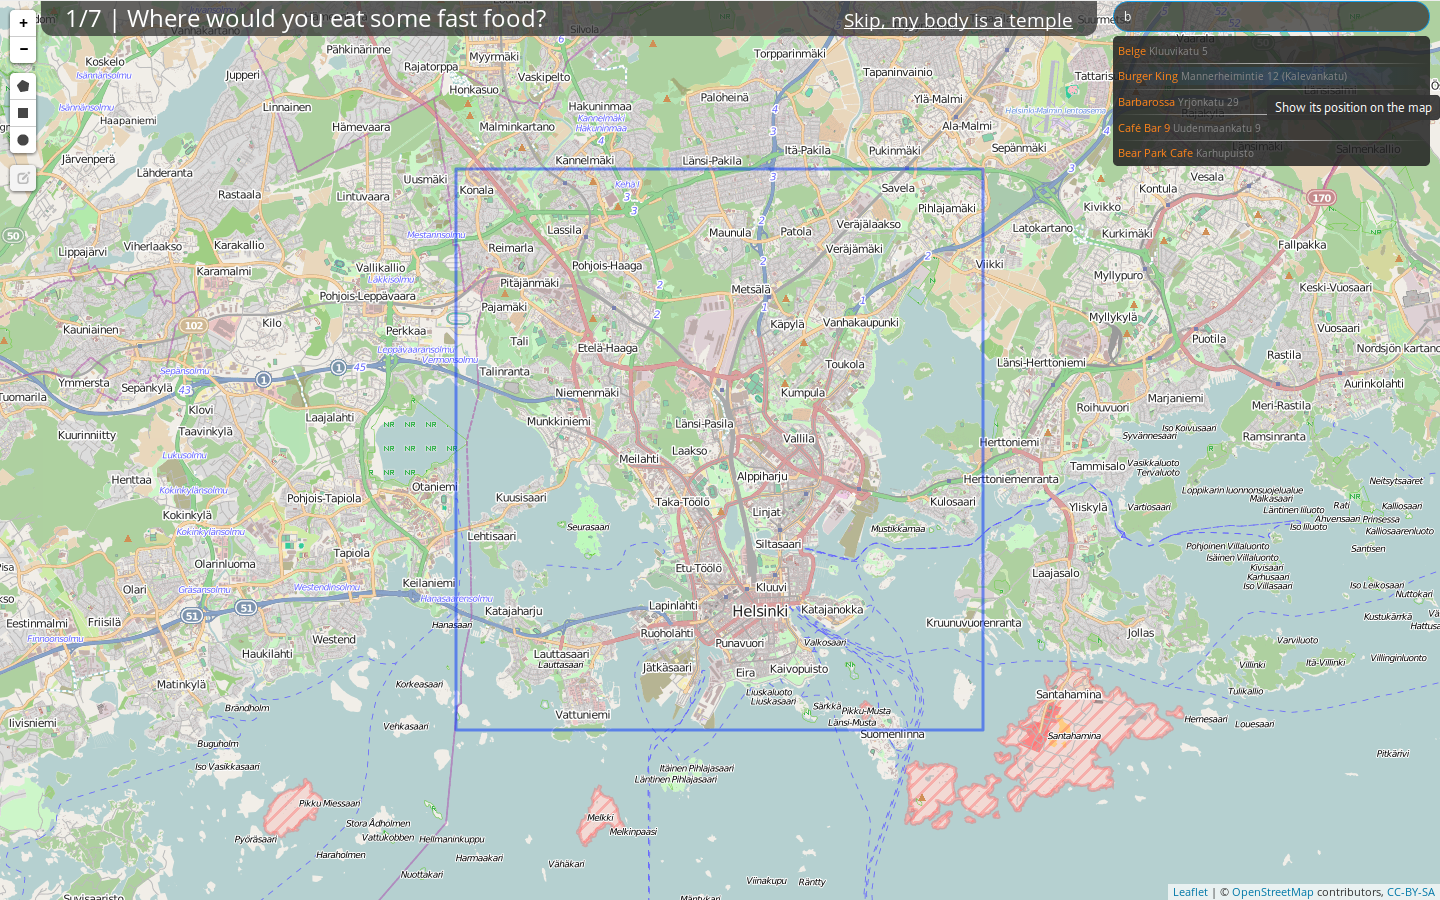
\includegraphics[width=\textwidth]{survey}
        \caption{The main screen of the survey.}
    \end{subfigure}

    \begin{subfigure}[b]{\textwidth}
        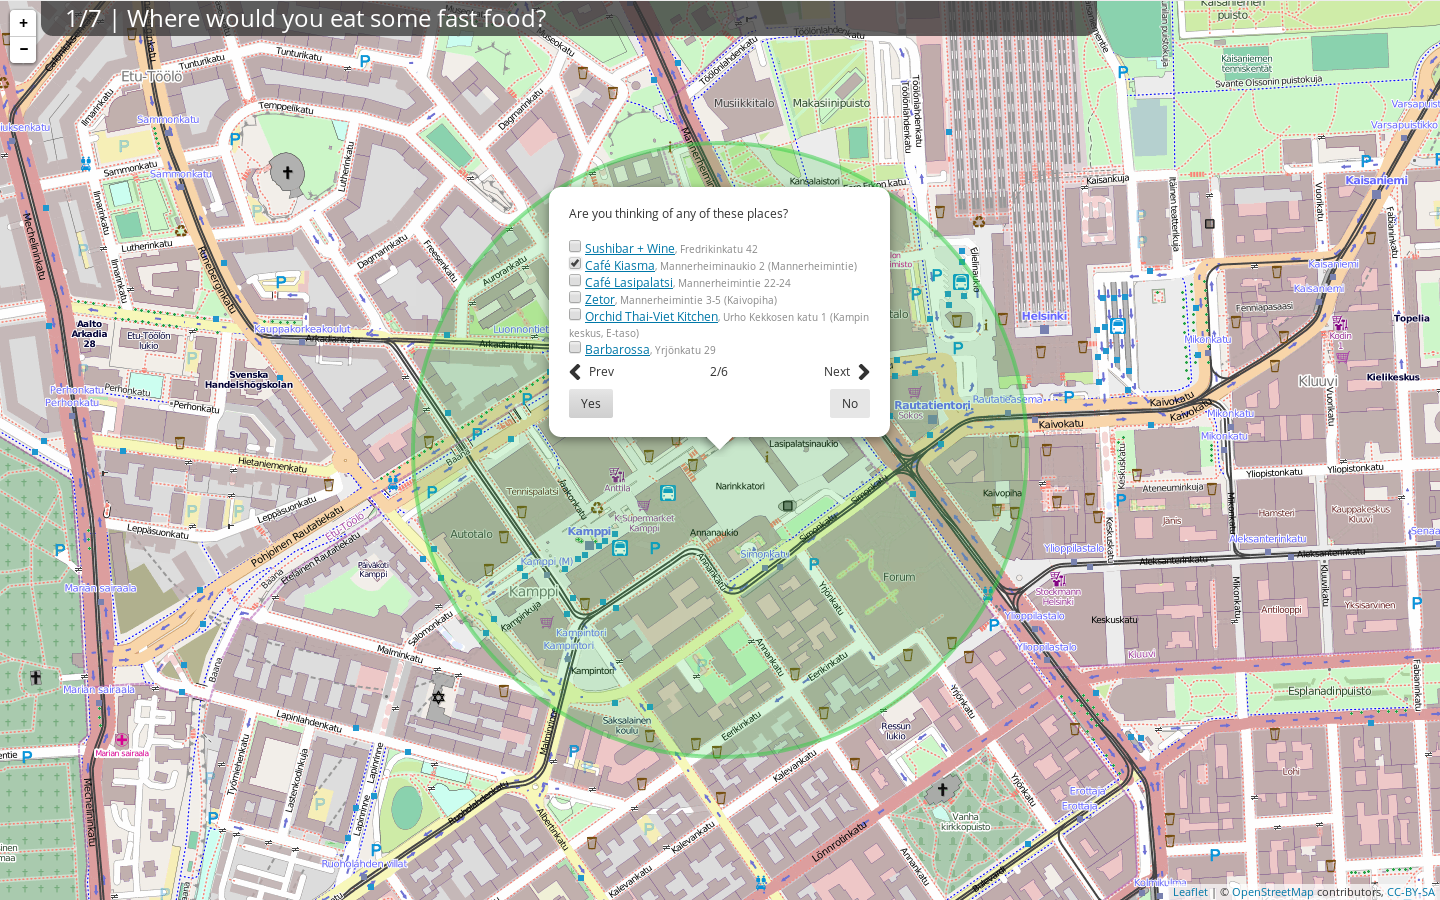
\includegraphics[width=\textwidth]{survey_venues}
        \caption{After an area have been drawn, the answer can be refined by
        choosing relevant venues from the dataset.}
    \end{subfigure}
    \caption{Website survey interface.\label{fig:survey}}
\end{figure}

However, we later realized that such information would still be difficult to
exploit. Thus we modified the website to collect another kind of data. Namely,
we hand picked eight neighborhoods in Paris, presented in
\autoref{tab:district}. And we asked international acquaintances to give us
similar places in the city where they have lived for some years and that they
know well. We obtained answers in Barcelona, New York, Paris, Rome, San
Francisco, and Washington DC. The answers were slightly altered so that if more
than one person provided answers for one city, the answers were merged.

\begin{table}[ht]
	\centering
	\begin{tabularx}{\textwidth}{lX}
		\toprule
		Name & Description \\
		\midrule
		Golden triangle & Near the Champs-Élysée, it is home of prestigious fashion shops (like Gucci or LVMH) and luxurious palaces (such as Ritz, Georges V or Carlton). \\
		Quartier Latin & A lot of top higher education institutions which draw plenty of reveller students. \\
		Pigalle & The historical red light district. \\
		Montmartre & Touristic spot as well as artsy district. \\
		Official & Here are gathered many official buildings such as the presidential palace, the national parliament and various ministries. \\
		Le Marais & It has welcomed many minorities throughout history, the last one being homosexuals in the 80s. \\
		16\textsuperscript{th} \enquote{arrondissement} & Real estate is expensive there and inhabitants are generally considered to be part of favored social class. \\
		The banks of the Seine & People can relax there during the weekend with friends or family, close to the nature. \\
		\bottomrule
	\end{tabularx}
	\caption[Ground truth neighborhoods]{List of Paris districts and accompanying
		descriptions. Participants in the study were asked to identify up to~5 most
	similar districts in their own city.\label{tab:district}}
\end{table}
